\section[CASA]{Analyse computationnelle de scènes auditives (CASA)}

\begin{frame}{Codage par transformée}

$$y = C(x) \in \mathbb{R}^Y | x \in \mathbb{R}^{X} \tilde{x} = C^{-1}(y), P_e(x) \simeq P_e(\tilde{x})$$
\begin{itemize}
\item $C$ : Quantification adaptative d'un équivalent de la Transformée de Fourier à Court Terme (TFCT)
\item $P_e$ : Modélisation de la sensibilité aux déformations de la membrane basilaire\citenote{Zwicker}{}{}{}
\end{itemize}
Gain : $Y<<X$
Validation : écoute
\end{frame}

\begin{frame}{Transformée de Fourier à Court Terme (TFCT)}
$$ X[m, t] = \sum_{n = - \infty}^{\infty} x[n] w[n-t] \mathrm{e}^{\frac{-2 \mathrm{j}  \pi m n}{N}} $$
\end{frame}

\begin{frame}{Spectrogramme}
\begin{center}
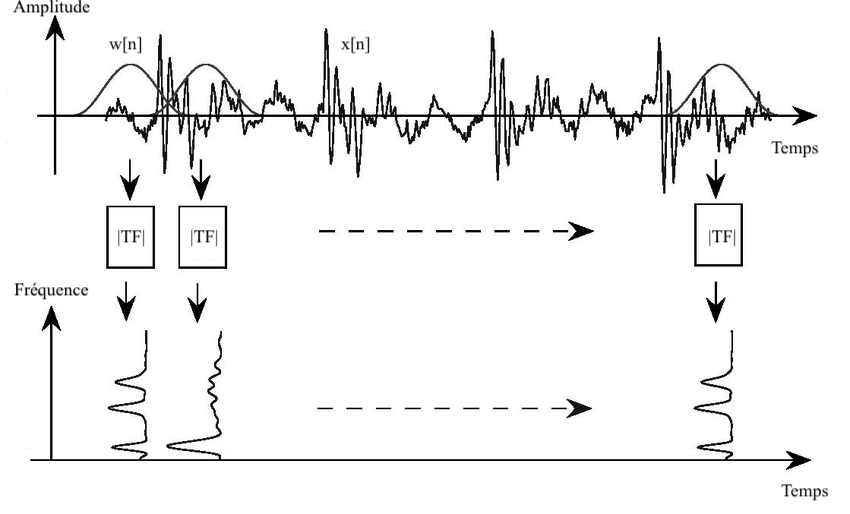
\includegraphics[width=.8\columnwidth]{figures/tfct} \\
\end{center}
Spectrogramme : $|X[m, t]|$
\end{frame}

\begin{frame}{Typologie des évènements sonores}
\begin{description}
  \item[parole] : sons voisés <a>, <o> / sons plosifs <pe>, <qe>;
  \item[communication animale] : hululement de chouettes / clics de localisation de chauve souris;
  \item[musique] : chant lyrique / percussions;
  \item[mécanique] : ventilation / marteau piqueur;
  \item[environnementaux] : vent faisant siffler des câbles / gouttes de pluie tombant sporadiquement.
\end{description}
\end{frame}

\begin{frame}{Compromis temps/fréquence}
\begin{center}
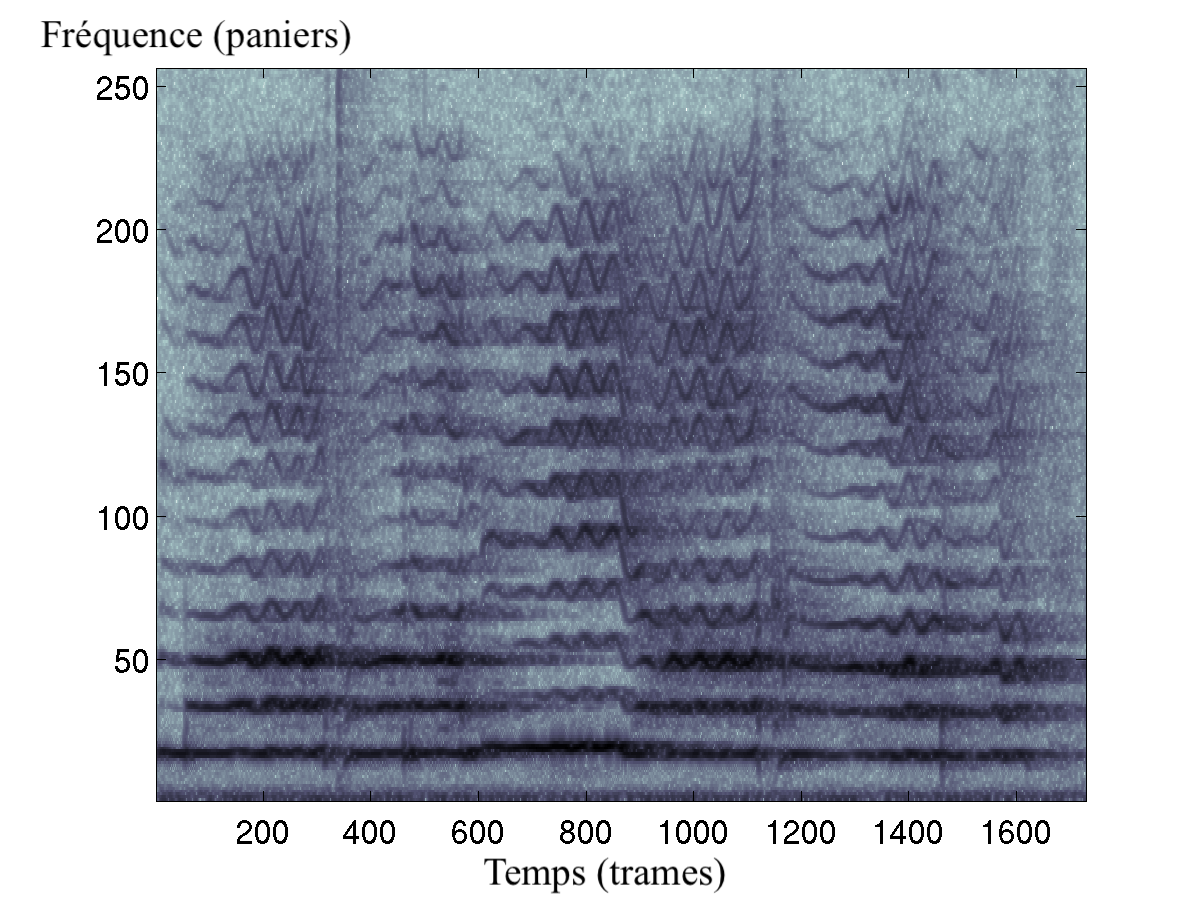
\includegraphics[width=.7\columnwidth]{figures/soloSpec} 
\end{center}
	$\hookrightarrow{}$ mitiger ce compromis imposée par l'approche court-terme par l'utilisation d'\alert{\textit{a prioris}} sur les sources d'intérêt.
\end{frame}

\begin{frame}{Analyse de Scènes Auditives Computationelle (CASA)}
L'ASA\footfullcite{bregman1994auditory} étudie l'ensemble de traitements perceptifs permettant
\begin{itemize}
\item d'isoler les informations émanant d'\structure{entités} sonores distinctes,
\item de les organiser en un tout cohérent.
\item à l'aide de processus \structure{\og primitifs \fg} et \structure{\og séquentiels \fg}.
\end{itemize}
L'Analyse de Scènes Auditives Computationnelle (CASA)\fullcitenote{wang2016casa} se propose de mettre en \oe~euvre ces critères pour inférer une organisation perceptuellement valide de la scène sonore.
\end{frame}

\begin{frame}{Processus ASA \og primitifs \fg}
\begin{description}
\item[\alert<2>{continuité}] : les propriétés d'un son isolé tendent à se modifier lentement et de façon continue
\item[harmonicité] : lorsqu'un corps sonore vibre à une période répétée, ses vibrations donnent naissance à un motif acoustique dont les fréquences des composants sont des multiples d'une même fréquence fondamentale;
\item[...]
\end{description}
\end{frame}

\begin{frame}{Modèle sinusoïdal à long terme}
\only<1>{
$$
x[n]=\sum_{l=1}^{L} a_{l}[n] \sin \left(\frac{2 \pi}{F_{s}} f_{l}[n] \cdot n + \Phi_k \right)
$$
$a_{l}[n]$ et $f_{l}[n]$ sont des signaux contrôlant respectivement l'amplitude et la phase des $L$ oscillateurs composant le modèle.
}
\only<2>{mettre le son et la figure} %http://webpages.mcgill.ca/staff/Group2/abregm1/web/snd/Track24.mp3
\end{frame}

\begin{tikzpicture}[
nonterminal/.append style={join=by ->},
tip/.style={->,shorten >=1pt},every join/.style={rounded corners},
terminal/.style={
% The shape:
rectangle,minimum size=6mm,rounded corners=1mm,
% The rest
very thick,draw=black!50,
top color=white,bottom color=black!10,
font=\ttfamily},
point/.style={circle,fill=black,minimum size=2pt},
%every node/.style=draw,
line/.style ={draw, thick, -latex',shorten
  >=2pt}]



  \begin{tabular}{ccc}
    (a) & (b) & (c)  \\
  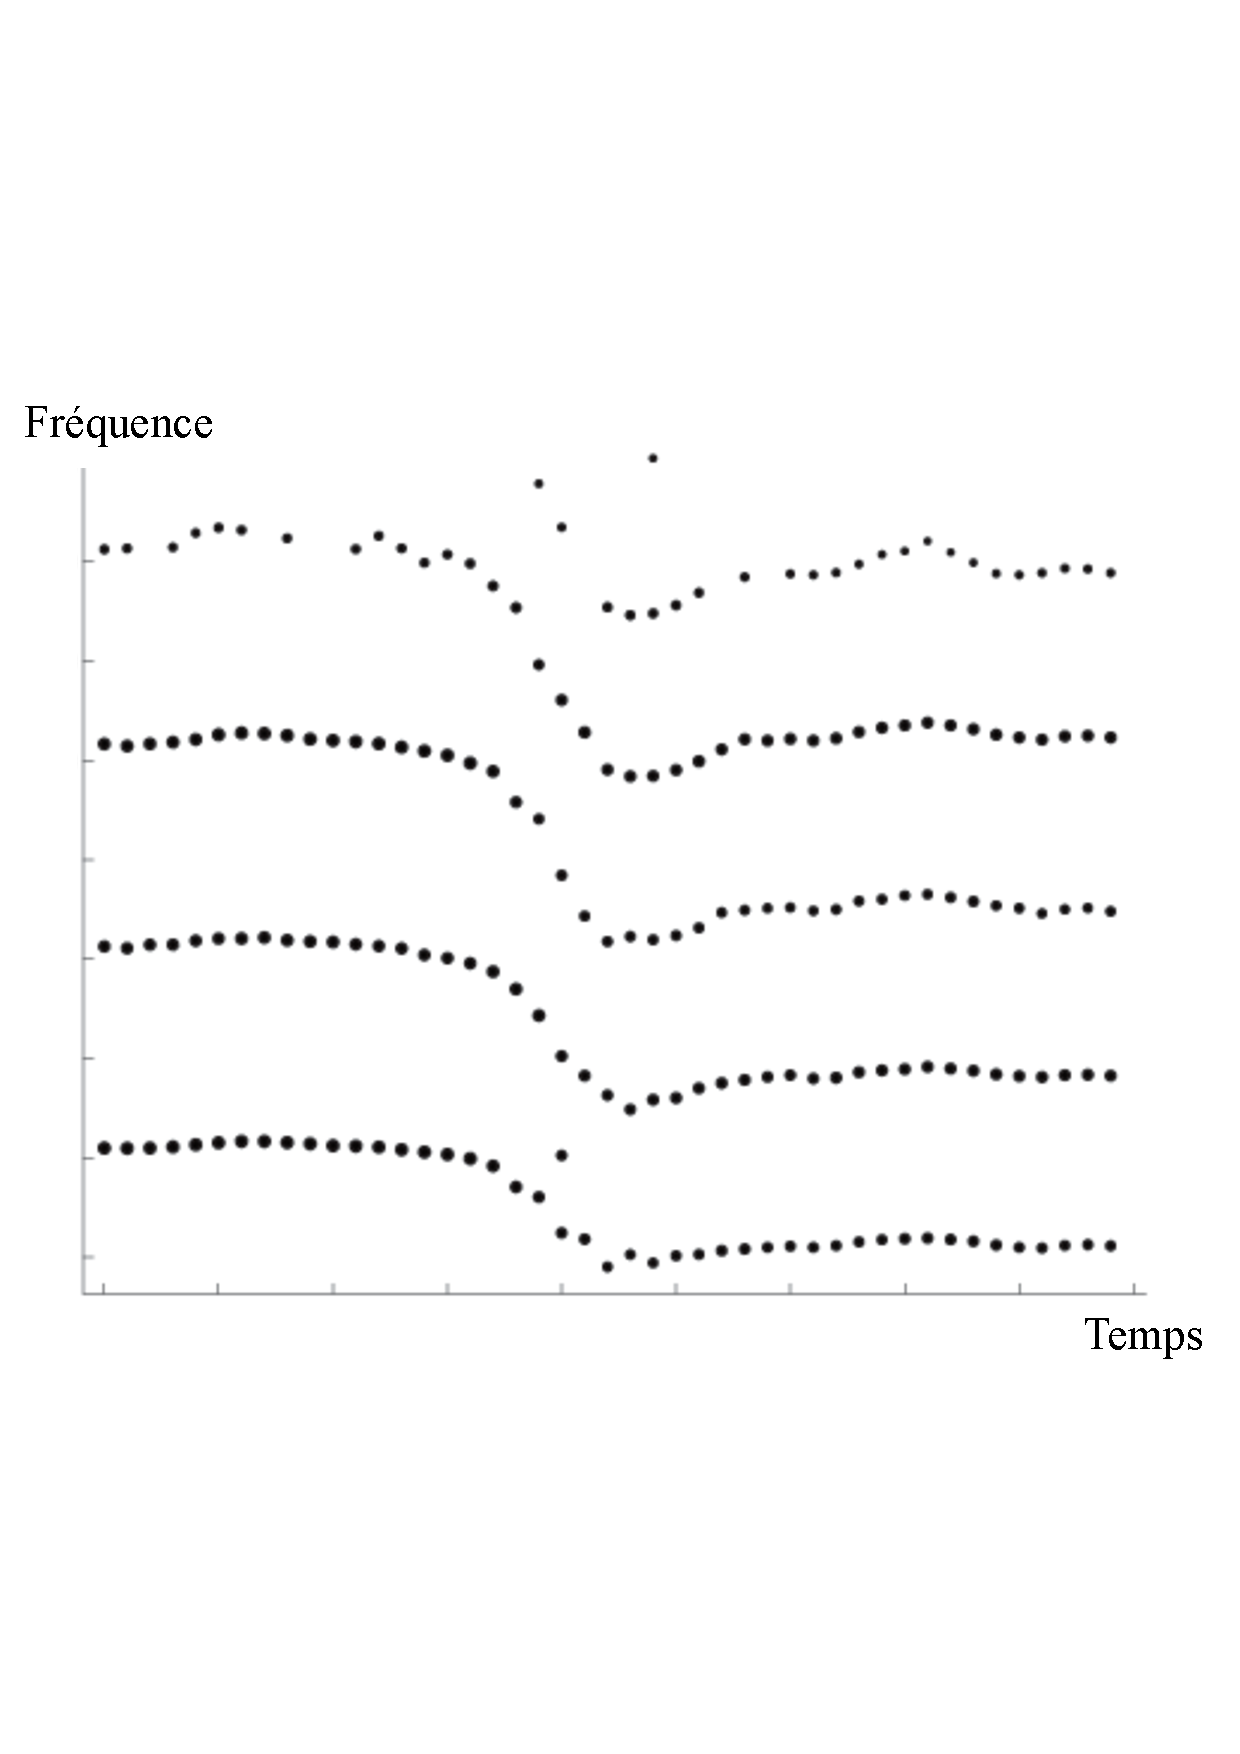
\includegraphics[width=.3\textwidth]{voice_1024_512xp} &
  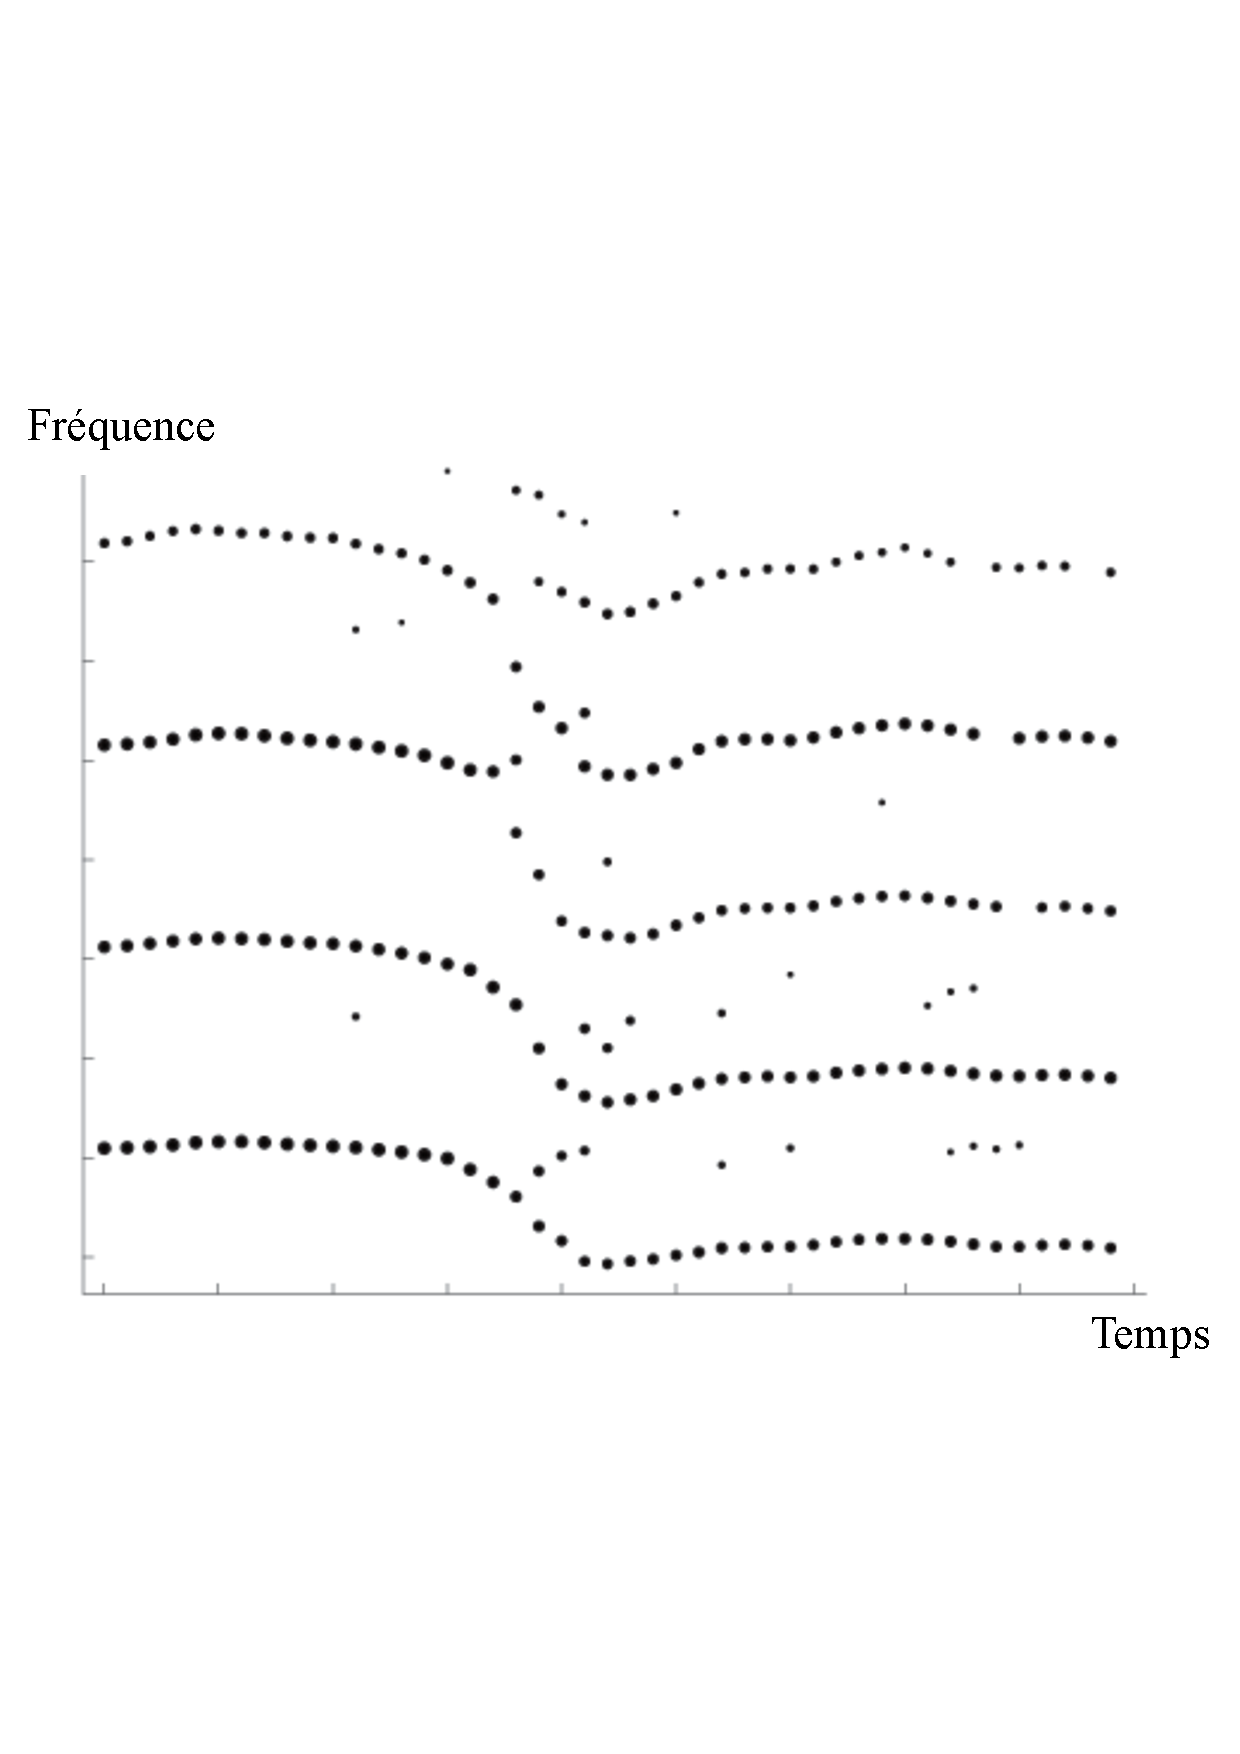
\includegraphics[width=.3\textwidth]{voice_2048_512xp} &
  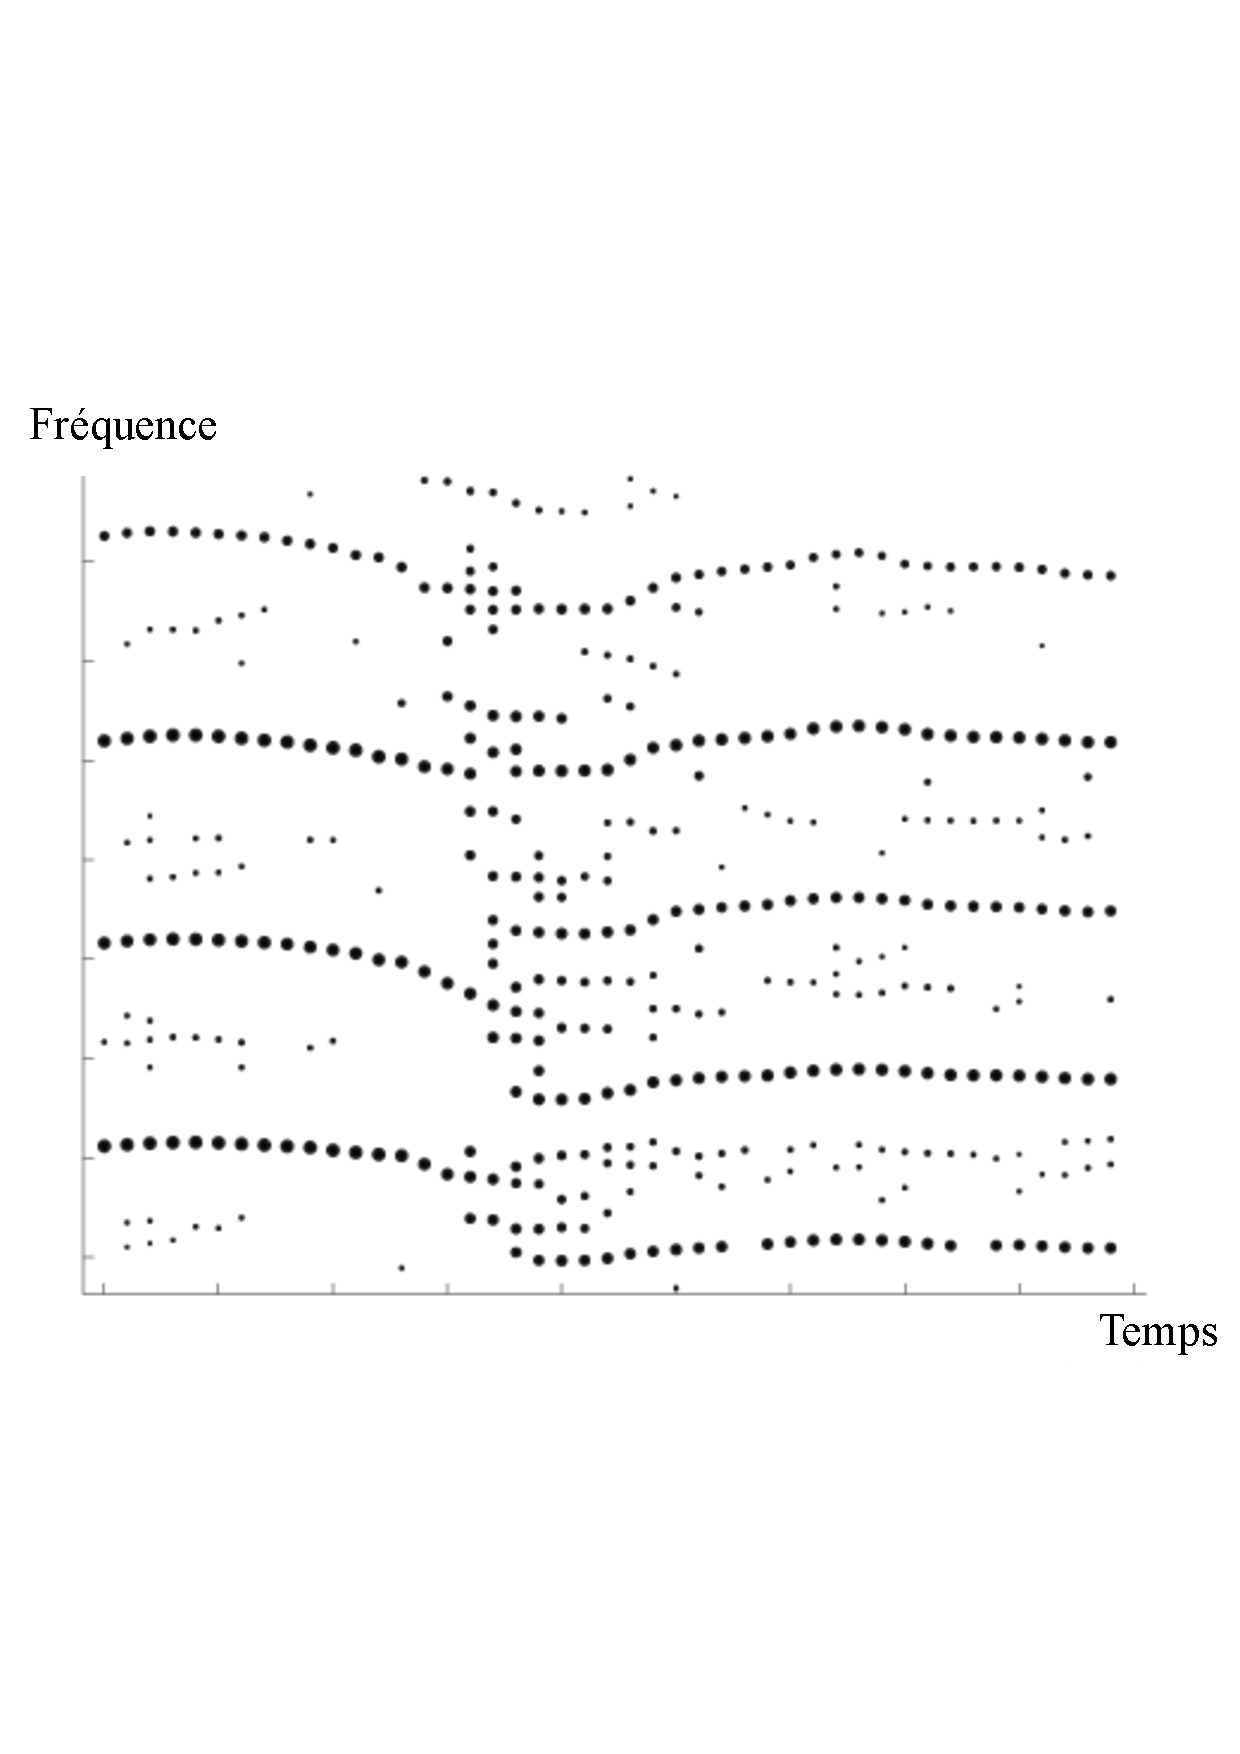
\includegraphics[width=.3\textwidth]{voice_4096_512xp} \\
\end{tabular}
  \caption{Influence de la taille de fenêtre de la tfct utilisée pour estimer un modèle sinusoïdal à court terme d'un glissando de trombone. De gauche à droite, la taille est de 25 (a), 50 (b), et 100 ms (c), pour un pas d'avancement de 10 ms. Chaque point correspond  à une composante à court terme $p_{t, c}$ et sa taille est fonction de l'amplitude de la composante $a_{t, c}$.}

  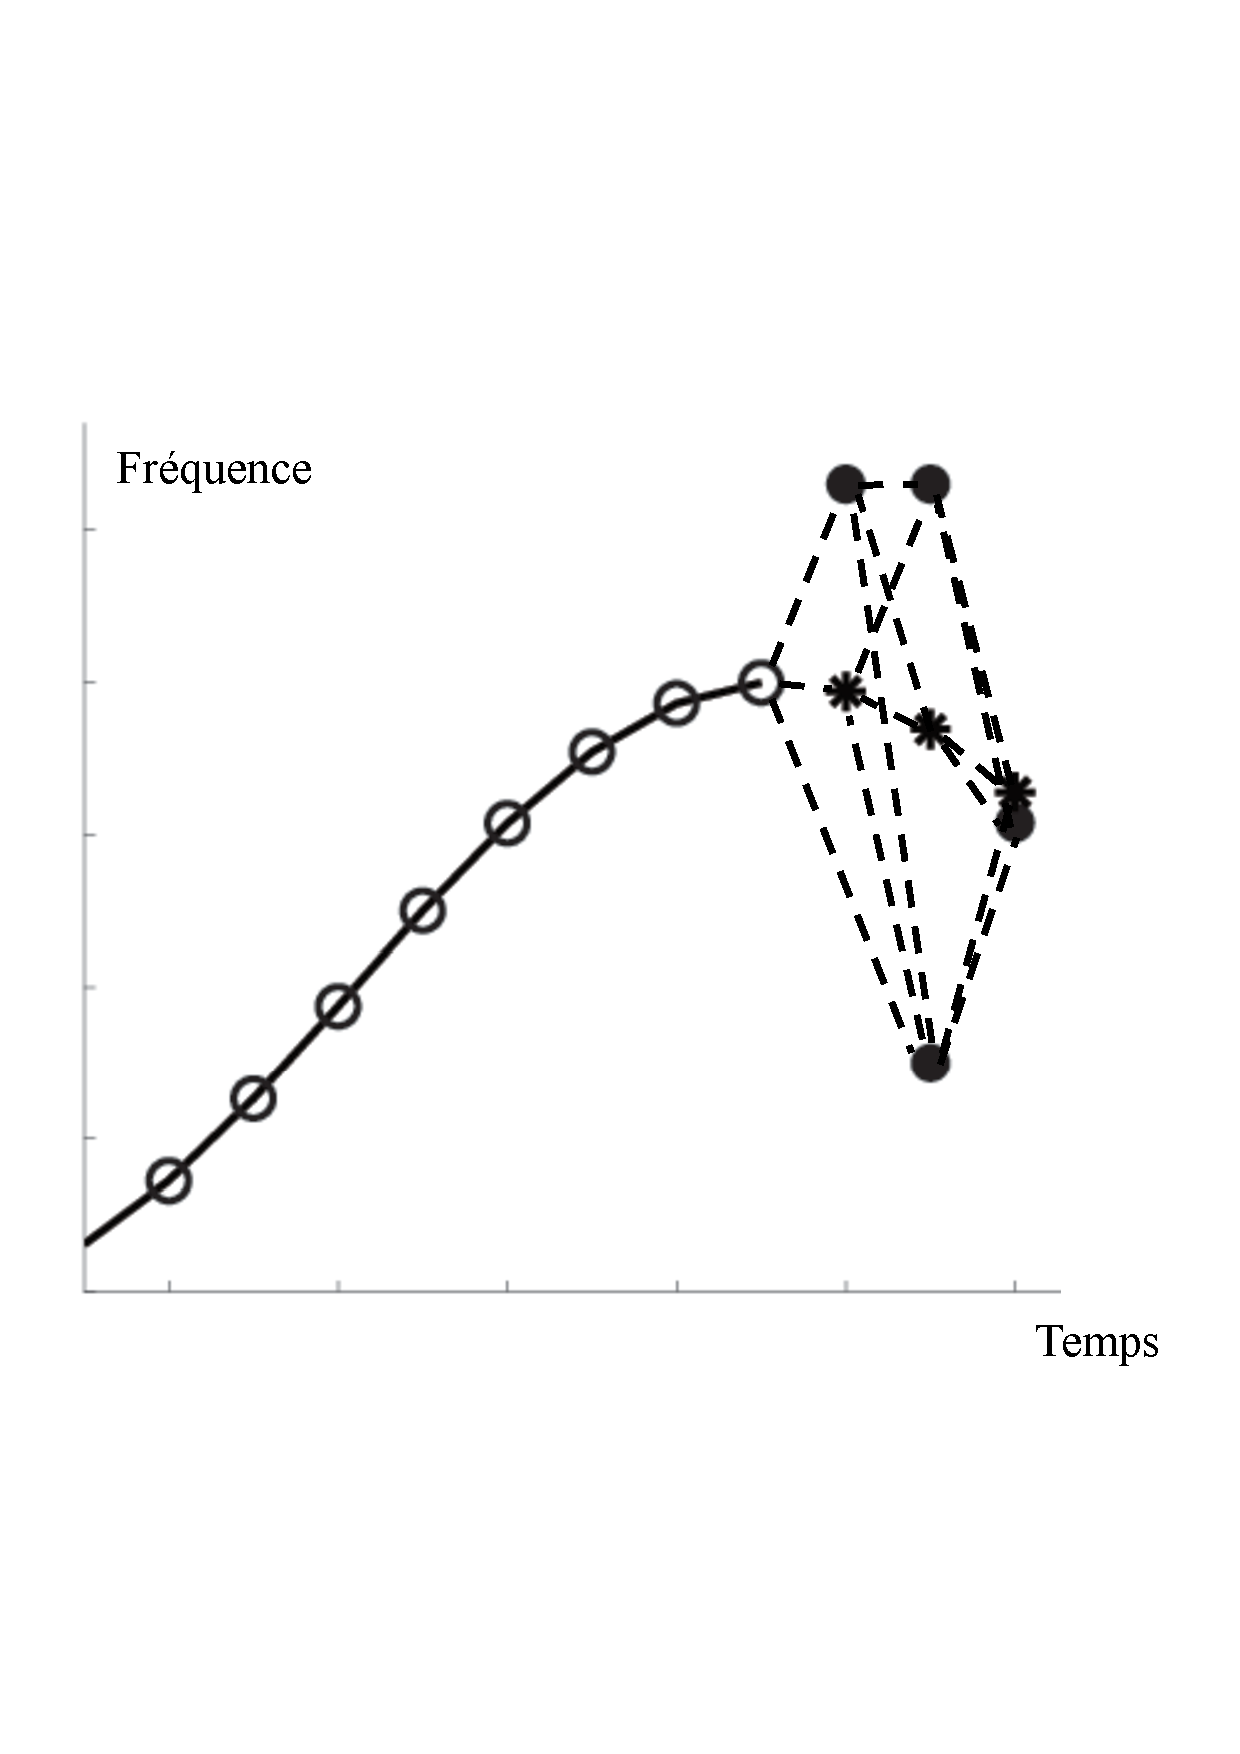
\includegraphics[width=.5\textwidth]{trackingxp2xp2}
\fullcitenote{lagrangeTaslp06}

\begin{tabular}{ccc}
    (a) & (b) & (c)  \\
  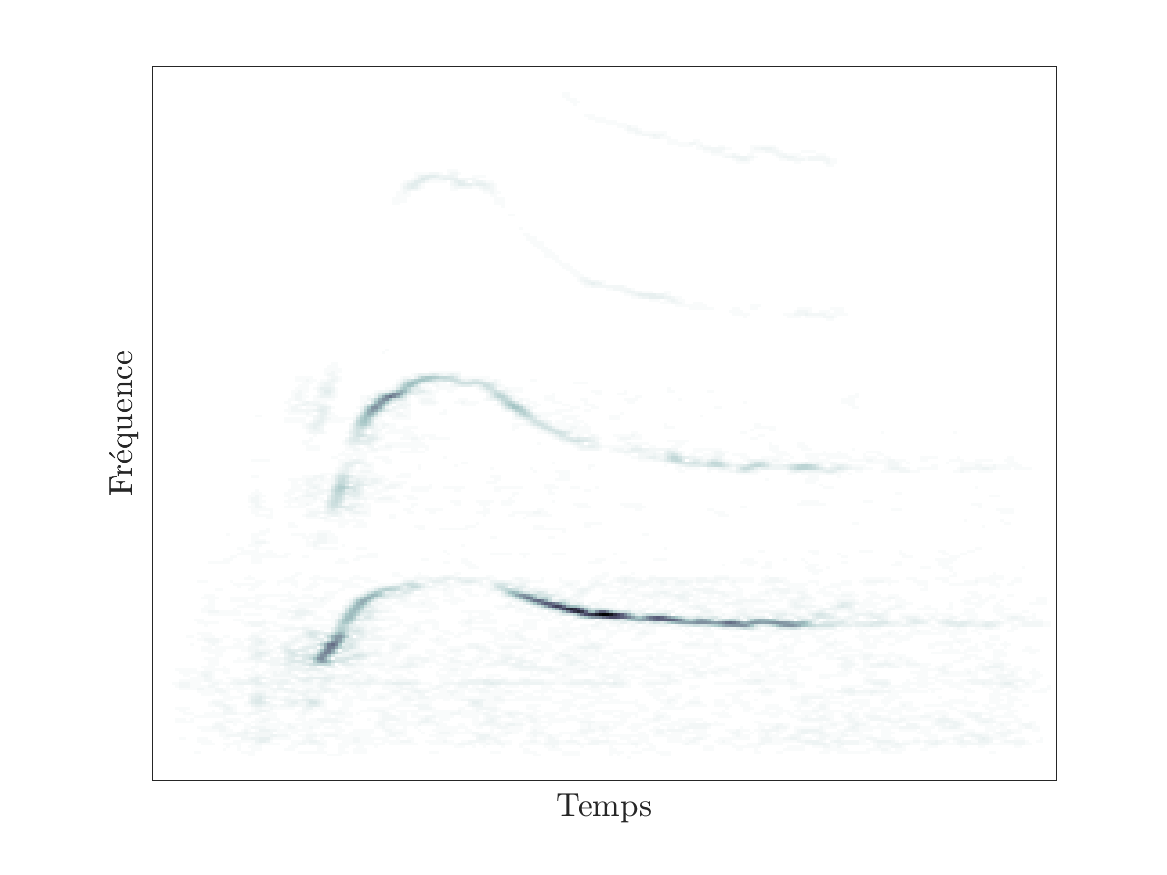
\includegraphics[width=.333\textwidth]{orcaOriSpec} &
  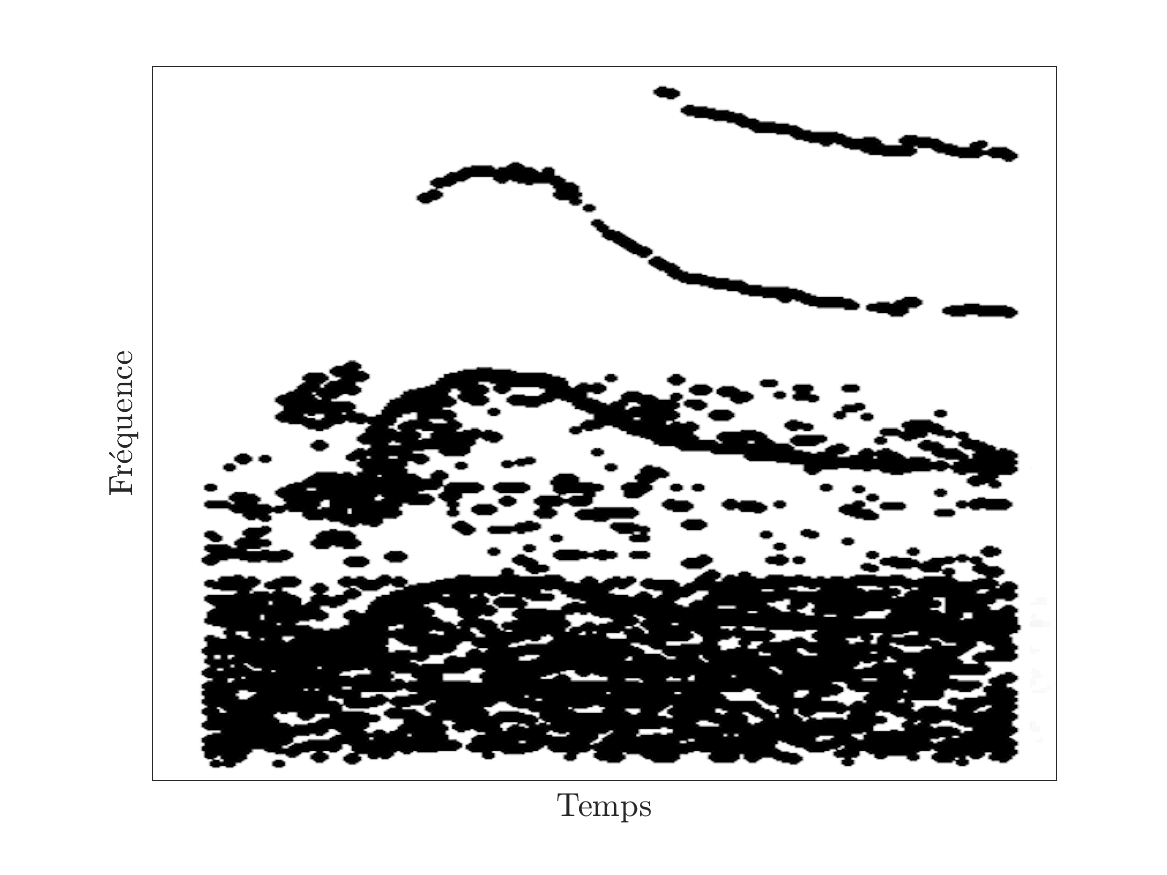
\includegraphics[width=.333\textwidth]{orcaSin} &
  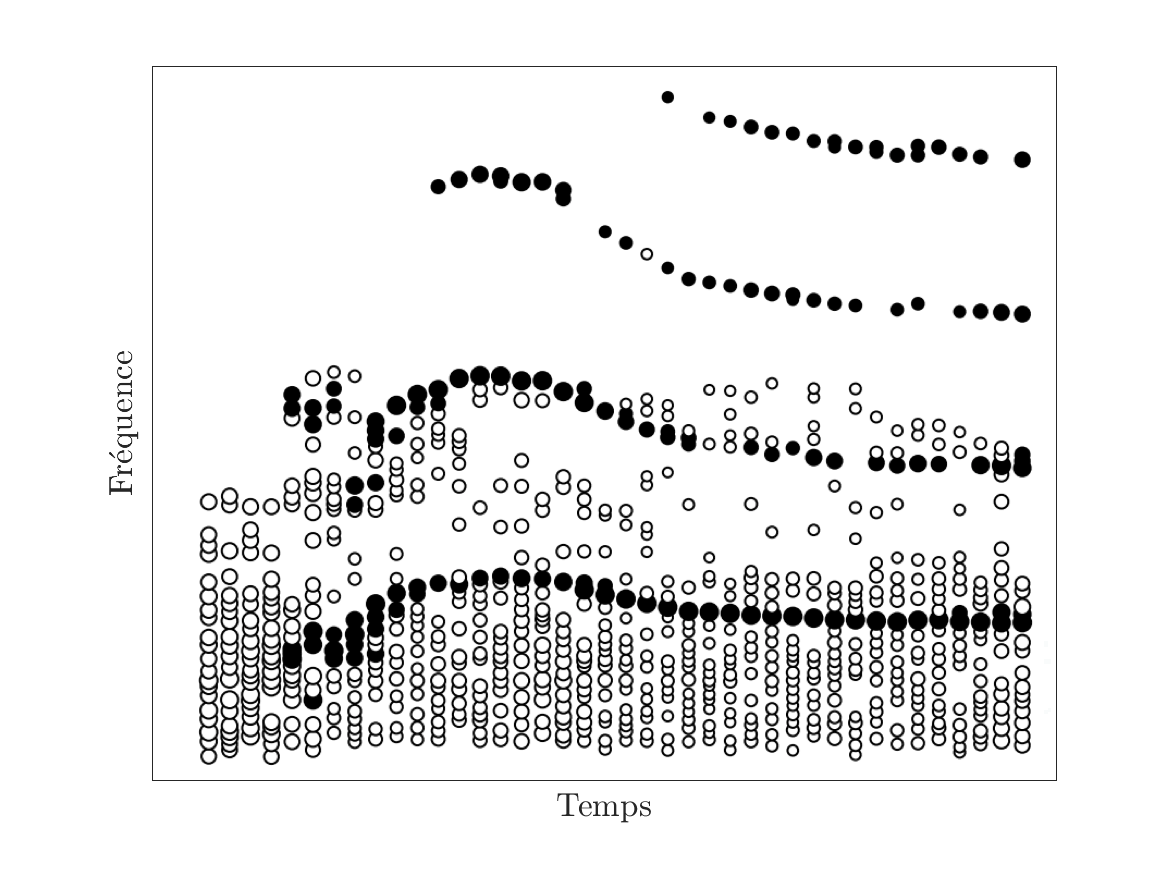
\includegraphics[width=.333\textwidth]{orcaSep} \\
\end{tabular}

Exemple ASA modulations

Modele sinusoidal long terme

Analyse a court terme

Tracking lentement predictible et ne pas générer de hautes fréquences

critère de continuation un critère de formation de sources parmi d'autres

asa

criteres instantanés

critères 

casa

asa  (ref ellis)

normalized cuts

\begin{frame}{Processus ASA \og séquentiels \fg}
\begin{description}
\item[proximité] : des éléments proches les uns des autres sur le plan temps/fréquence ont tendance à être groupés ensemble
\item[similarité] : des éléments qui se ressemblent ont tendance à être groupés ensemble (timbre). 
\item[...]
\end{description}
\end{frame}

houle

constat

long terme mais court terme :/

Ca ne marche pas, mais je peux expliquer pourquoi
Ca marche, mais je ne peux pas vraiment dire pourquoi
